% Options for packages loaded elsewhere
\PassOptionsToPackage{unicode}{hyperref}
\PassOptionsToPackage{hyphens}{url}
%
\documentclass[
]{article}
\usepackage{lmodern}
\usepackage{amsmath}
\usepackage{ifxetex,ifluatex}
\ifnum 0\ifxetex 1\fi\ifluatex 1\fi=0 % if pdftex
  \usepackage[T1]{fontenc}
  \usepackage[utf8]{inputenc}
  \usepackage{textcomp} % provide euro and other symbols
  \usepackage{amssymb}
\else % if luatex or xetex
  \usepackage{unicode-math}
  \defaultfontfeatures{Scale=MatchLowercase}
  \defaultfontfeatures[\rmfamily]{Ligatures=TeX,Scale=1}
\fi
% Use upquote if available, for straight quotes in verbatim environments
\IfFileExists{upquote.sty}{\usepackage{upquote}}{}
\IfFileExists{microtype.sty}{% use microtype if available
  \usepackage[]{microtype}
  \UseMicrotypeSet[protrusion]{basicmath} % disable protrusion for tt fonts
}{}
\makeatletter
\@ifundefined{KOMAClassName}{% if non-KOMA class
  \IfFileExists{parskip.sty}{%
    \usepackage{parskip}
  }{% else
    \setlength{\parindent}{0pt}
    \setlength{\parskip}{6pt plus 2pt minus 1pt}}
}{% if KOMA class
  \KOMAoptions{parskip=half}}
\makeatother
\usepackage{xcolor}
\IfFileExists{xurl.sty}{\usepackage{xurl}}{} % add URL line breaks if available
\IfFileExists{bookmark.sty}{\usepackage{bookmark}}{\usepackage{hyperref}}
\hypersetup{
  pdftitle={Gestion de Portefeuille},
  pdfauthor={Patrick Hénaff},
  hidelinks,
  pdfcreator={LaTeX via pandoc}}
\urlstyle{same} % disable monospaced font for URLs
\usepackage[margin=1in]{geometry}
\usepackage{color}
\usepackage{fancyvrb}
\newcommand{\VerbBar}{|}
\newcommand{\VERB}{\Verb[commandchars=\\\{\}]}
\DefineVerbatimEnvironment{Highlighting}{Verbatim}{commandchars=\\\{\}}
% Add ',fontsize=\small' for more characters per line
\usepackage{framed}
\definecolor{shadecolor}{RGB}{248,248,248}
\newenvironment{Shaded}{\begin{snugshade}}{\end{snugshade}}
\newcommand{\AlertTok}[1]{\textcolor[rgb]{0.94,0.16,0.16}{#1}}
\newcommand{\AnnotationTok}[1]{\textcolor[rgb]{0.56,0.35,0.01}{\textbf{\textit{#1}}}}
\newcommand{\AttributeTok}[1]{\textcolor[rgb]{0.77,0.63,0.00}{#1}}
\newcommand{\BaseNTok}[1]{\textcolor[rgb]{0.00,0.00,0.81}{#1}}
\newcommand{\BuiltInTok}[1]{#1}
\newcommand{\CharTok}[1]{\textcolor[rgb]{0.31,0.60,0.02}{#1}}
\newcommand{\CommentTok}[1]{\textcolor[rgb]{0.56,0.35,0.01}{\textit{#1}}}
\newcommand{\CommentVarTok}[1]{\textcolor[rgb]{0.56,0.35,0.01}{\textbf{\textit{#1}}}}
\newcommand{\ConstantTok}[1]{\textcolor[rgb]{0.00,0.00,0.00}{#1}}
\newcommand{\ControlFlowTok}[1]{\textcolor[rgb]{0.13,0.29,0.53}{\textbf{#1}}}
\newcommand{\DataTypeTok}[1]{\textcolor[rgb]{0.13,0.29,0.53}{#1}}
\newcommand{\DecValTok}[1]{\textcolor[rgb]{0.00,0.00,0.81}{#1}}
\newcommand{\DocumentationTok}[1]{\textcolor[rgb]{0.56,0.35,0.01}{\textbf{\textit{#1}}}}
\newcommand{\ErrorTok}[1]{\textcolor[rgb]{0.64,0.00,0.00}{\textbf{#1}}}
\newcommand{\ExtensionTok}[1]{#1}
\newcommand{\FloatTok}[1]{\textcolor[rgb]{0.00,0.00,0.81}{#1}}
\newcommand{\FunctionTok}[1]{\textcolor[rgb]{0.00,0.00,0.00}{#1}}
\newcommand{\ImportTok}[1]{#1}
\newcommand{\InformationTok}[1]{\textcolor[rgb]{0.56,0.35,0.01}{\textbf{\textit{#1}}}}
\newcommand{\KeywordTok}[1]{\textcolor[rgb]{0.13,0.29,0.53}{\textbf{#1}}}
\newcommand{\NormalTok}[1]{#1}
\newcommand{\OperatorTok}[1]{\textcolor[rgb]{0.81,0.36,0.00}{\textbf{#1}}}
\newcommand{\OtherTok}[1]{\textcolor[rgb]{0.56,0.35,0.01}{#1}}
\newcommand{\PreprocessorTok}[1]{\textcolor[rgb]{0.56,0.35,0.01}{\textit{#1}}}
\newcommand{\RegionMarkerTok}[1]{#1}
\newcommand{\SpecialCharTok}[1]{\textcolor[rgb]{0.00,0.00,0.00}{#1}}
\newcommand{\SpecialStringTok}[1]{\textcolor[rgb]{0.31,0.60,0.02}{#1}}
\newcommand{\StringTok}[1]{\textcolor[rgb]{0.31,0.60,0.02}{#1}}
\newcommand{\VariableTok}[1]{\textcolor[rgb]{0.00,0.00,0.00}{#1}}
\newcommand{\VerbatimStringTok}[1]{\textcolor[rgb]{0.31,0.60,0.02}{#1}}
\newcommand{\WarningTok}[1]{\textcolor[rgb]{0.56,0.35,0.01}{\textbf{\textit{#1}}}}
\usepackage{graphicx}
\makeatletter
\def\maxwidth{\ifdim\Gin@nat@width>\linewidth\linewidth\else\Gin@nat@width\fi}
\def\maxheight{\ifdim\Gin@nat@height>\textheight\textheight\else\Gin@nat@height\fi}
\makeatother
% Scale images if necessary, so that they will not overflow the page
% margins by default, and it is still possible to overwrite the defaults
% using explicit options in \includegraphics[width, height, ...]{}
\setkeys{Gin}{width=\maxwidth,height=\maxheight,keepaspectratio}
% Set default figure placement to htbp
\makeatletter
\def\fps@figure{htbp}
\makeatother
\setlength{\emergencystretch}{3em} % prevent overfull lines
\providecommand{\tightlist}{%
  \setlength{\itemsep}{0pt}\setlength{\parskip}{0pt}}
\setcounter{secnumdepth}{-\maxdimen} % remove section numbering
\usepackage[utf8]{inputenc}
\usepackage{booktabs}
\usepackage{longtable}
\usepackage{array}
\usepackage{multirow}
\usepackage{wrapfig}
\usepackage{float}
\usepackage{colortbl}
\usepackage{pdflscape}
\usepackage{tabu}
\usepackage{threeparttable}
\usepackage{threeparttablex}
\usepackage[normalem]{ulem}
\usepackage{makecell}
\usepackage{xcolor}
\ifluatex
  \usepackage{selnolig}  % disable illegal ligatures
\fi

\title{Gestion de Portefeuille}
\usepackage{etoolbox}
\makeatletter
\providecommand{\subtitle}[1]{% add subtitle to \maketitle
  \apptocmd{\@title}{\par {\large #1 \par}}{}{}
}
\makeatother
\subtitle{TP-4: Simulation d'une gestion selon un Budget Risque}
\author{Patrick Hénaff}
\date{Février-Mars 2021}

\begin{document}
\maketitle

L'objet de ce TP est de se familiariser avec les packages de
``backtesting'' disponibles dans R. pour cela, on propose de reproduire
une analyse réalisée avec le package ``riskParityPortfolio,'' mais en
utilisant un nouveau jeu de données, et en portant quelques
modifications à l'exemple proposé.

\hypertarget{le-package-riskparityportfolio}{%
\subsection{Le package
``riskParityPortfolio''}\label{le-package-riskparityportfolio}}

L'exemple suivant est présenté dans la vignette
\url{https://cran.r-project.org/web/packages/riskParityPortfolio/vignettes/RiskParityPortfolio.html}

\begin{Shaded}
\begin{Highlighting}[]
\CommentTok{\# données de Yahoo! Finance}
\NormalTok{faang\_data }\OtherTok{\textless{}{-}} \FunctionTok{stockDataDownload}\NormalTok{(}\FunctionTok{c}\NormalTok{(}\StringTok{"GOOG"}\NormalTok{, }\StringTok{"NFLX"}\NormalTok{, }\StringTok{"AAPL"}\NormalTok{, }\StringTok{"AMZN"}\NormalTok{, }\StringTok{"FB"}\NormalTok{),}
                                \AttributeTok{from =} \StringTok{"2014{-}01{-}01"}\NormalTok{, }\AttributeTok{to =} \StringTok{"2019{-}06{-}25"}\NormalTok{)}
\end{Highlighting}
\end{Shaded}

pour effectuer un backtest, on définit une fonction qui recoit en entrée
une liste de séries de type \texttt{xts}, et retourne un vecteur de
poids aloués à chaque actif. Chaque série de la liste a une colonne par
actif. Noter que la liste peut contenir autant de series que necessaire
pour exécuter l'algorithme d'allocation. Dans notre cas, on n'a besoin
que du cours de cloture ajusté. Cette fonction sera éxécutée de
multiples fois, selon les directives données dans la fonction de
simulation. Les fonctions présentées dans la documentation sont:

\begin{Shaded}
\begin{Highlighting}[]
\CommentTok{\# define portfolios to be backtested}
\CommentTok{\# risk parity portfolio}
\NormalTok{risk\_parity }\OtherTok{\textless{}{-}} \ControlFlowTok{function}\NormalTok{(dataset) \{}
\NormalTok{  prices }\OtherTok{\textless{}{-}}\NormalTok{ dataset}\SpecialCharTok{$}\NormalTok{adjusted}
\NormalTok{  log\_returns }\OtherTok{\textless{}{-}} \FunctionTok{diff}\NormalTok{(}\FunctionTok{log}\NormalTok{(prices))[}\SpecialCharTok{{-}}\DecValTok{1}\NormalTok{]}
  \FunctionTok{return}\NormalTok{(}\FunctionTok{riskParityPortfolio}\NormalTok{(}\FunctionTok{cov}\NormalTok{(log\_returns))}\SpecialCharTok{$}\NormalTok{w)}
\NormalTok{\}}
\end{Highlighting}
\end{Shaded}

\begin{Shaded}
\begin{Highlighting}[]
\CommentTok{\# tangency portfolio (maximum sharpe ratio)}
\NormalTok{max\_sharpe\_ratio }\OtherTok{\textless{}{-}} \ControlFlowTok{function}\NormalTok{(dataset) \{}
\NormalTok{    prices }\OtherTok{\textless{}{-}}\NormalTok{ dataset}\SpecialCharTok{$}\NormalTok{adjusted}
\NormalTok{    log\_returns }\OtherTok{\textless{}{-}} \FunctionTok{diff}\NormalTok{(}\FunctionTok{log}\NormalTok{(prices))[}\SpecialCharTok{{-}}\DecValTok{1}\NormalTok{]}
\NormalTok{    N }\OtherTok{\textless{}{-}} \FunctionTok{ncol}\NormalTok{(prices)}
\NormalTok{    Sigma }\OtherTok{\textless{}{-}} \FunctionTok{cov}\NormalTok{(log\_returns)}
\NormalTok{    mu }\OtherTok{\textless{}{-}} \FunctionTok{colMeans}\NormalTok{(log\_returns)}
    \ControlFlowTok{if}\NormalTok{ (}\FunctionTok{all}\NormalTok{(mu }\SpecialCharTok{\textless{}=} \FloatTok{1e{-}8}\NormalTok{))}
        \FunctionTok{return}\NormalTok{(}\FunctionTok{rep}\NormalTok{(}\DecValTok{0}\NormalTok{, N))}
\NormalTok{    Dmat }\OtherTok{\textless{}{-}} \DecValTok{2} \SpecialCharTok{*}\NormalTok{ Sigma}
\NormalTok{    Amat }\OtherTok{\textless{}{-}} \FunctionTok{diag}\NormalTok{(N)}
\NormalTok{    Amat }\OtherTok{\textless{}{-}} \FunctionTok{cbind}\NormalTok{(mu, Amat)}
\NormalTok{    bvec }\OtherTok{\textless{}{-}} \FunctionTok{c}\NormalTok{(}\DecValTok{1}\NormalTok{, }\FunctionTok{rep}\NormalTok{(}\DecValTok{0}\NormalTok{, N))}
\NormalTok{    dvec }\OtherTok{\textless{}{-}} \FunctionTok{rep}\NormalTok{(}\DecValTok{0}\NormalTok{, N)}
\NormalTok{    res }\OtherTok{\textless{}{-}} \FunctionTok{solve.QP}\NormalTok{(}\AttributeTok{Dmat =}\NormalTok{ Dmat, }\AttributeTok{dvec =}\NormalTok{ dvec, }\AttributeTok{Amat =}\NormalTok{ Amat, }\AttributeTok{bvec =}\NormalTok{ bvec, }\AttributeTok{meq =} \DecValTok{1}\NormalTok{)}
\NormalTok{    w }\OtherTok{\textless{}{-}}\NormalTok{ res}\SpecialCharTok{$}\NormalTok{solution}
    \FunctionTok{return}\NormalTok{(w}\SpecialCharTok{/}\FunctionTok{sum}\NormalTok{(w))}
\NormalTok{\}}
\end{Highlighting}
\end{Shaded}

Le backtest lui-même est défini par les paramètres suivants:

\begin{itemize}
\tightlist
\item
  Fenêtre de données historiques à utiliser dans chaque calcul: 240
  jours
\item
  Recalcul des poids tous les 60 jours
\item
  Rééquilibrage du portefeuille tous les 60 jours.
\end{itemize}

On effectue parfois des rééquilibrages entre deux recalculs des poids,
pour prendre en compte les mouvements de marché.

\begin{Shaded}
\begin{Highlighting}[]
\CommentTok{\# call portfolioBacktest and benchmark against the uniform (1/N) portfolio}
\NormalTok{bt }\OtherTok{\textless{}{-}} \FunctionTok{portfolioBacktest}\NormalTok{(}\FunctionTok{list}\NormalTok{(}\StringTok{"risk parity portfolio"} \OtherTok{=}\NormalTok{ risk\_parity,}
                             \StringTok{"tangency portfolio"}    \OtherTok{=}\NormalTok{ max\_sharpe\_ratio),}
                        \FunctionTok{list}\NormalTok{(faang\_data),}
                        \AttributeTok{T\_rolling\_window =} \DecValTok{12}\SpecialCharTok{*}\DecValTok{20}\NormalTok{, }
                        \AttributeTok{optimize\_every =} \DecValTok{3}\SpecialCharTok{*}\DecValTok{20}\NormalTok{, }\AttributeTok{rebalance\_every =} \DecValTok{3}\SpecialCharTok{*}\DecValTok{20}\NormalTok{)}
\end{Highlighting}
\end{Shaded}

\begin{verbatim}
## 
##  [Backtesting 2 portfolios over 1 datasets (periodicity = daily data)]
\end{verbatim}

Les dates de recalcul:

\begin{Shaded}
\begin{Highlighting}[]
\FunctionTok{index}\NormalTok{(bt}\SpecialCharTok{$}\NormalTok{tangency}\SpecialCharTok{$}\NormalTok{data1}\SpecialCharTok{$}\NormalTok{w\_designed)}
\end{Highlighting}
\end{Shaded}

\begin{verbatim}
##  [1] "2014-12-12" "2015-03-12" "2015-06-08" "2015-09-01" "2015-11-25"
##  [6] "2016-02-24" "2016-05-19" "2016-08-15" "2016-11-08" "2017-02-06"
## [11] "2017-05-03" "2017-07-28" "2017-10-23" "2018-01-19" "2018-04-17"
## [16] "2018-07-12" "2018-10-05" "2019-01-03" "2019-04-01"
\end{verbatim}

Résumé des performances des deux styles de gestion:

\begin{Shaded}
\begin{Highlighting}[]
\FunctionTok{kable}\NormalTok{(}\FunctionTok{backtestSummary}\NormalTok{(bt)}\SpecialCharTok{$}\NormalTok{performance, }\StringTok{"latex"}\NormalTok{, }\AttributeTok{booktabs=}\NormalTok{T)}
\end{Highlighting}
\end{Shaded}

\begin{tabular}{lrr}
\toprule
  & risk parity portfolio & tangency portfolio\\
\midrule
Sharpe ratio & 1.3800143 & 0.8787601\\
max drawdown & 0.3062046 & 0.3516856\\
annual return & 0.3117199 & 0.2324204\\
annual volatility & 0.2258817 & 0.2644867\\
Sterling ratio & 1.0180120 & 0.6608755\\
\addlinespace
Omega ratio & 1.2710283 & 1.1793761\\
ROT (bps) & 8310.1222983 & 793.0197047\\
VaR (0.95) & 0.0236911 & 0.0274712\\
CVaR (0.95) & 0.0346191 & 0.0403706\\
cpu time & 0.0122105 & 0.0042632\\
\addlinespace
failure rate & 0.0000000 & 0.0000000\\
\bottomrule
\end{tabular}

\begin{figure}
\centering
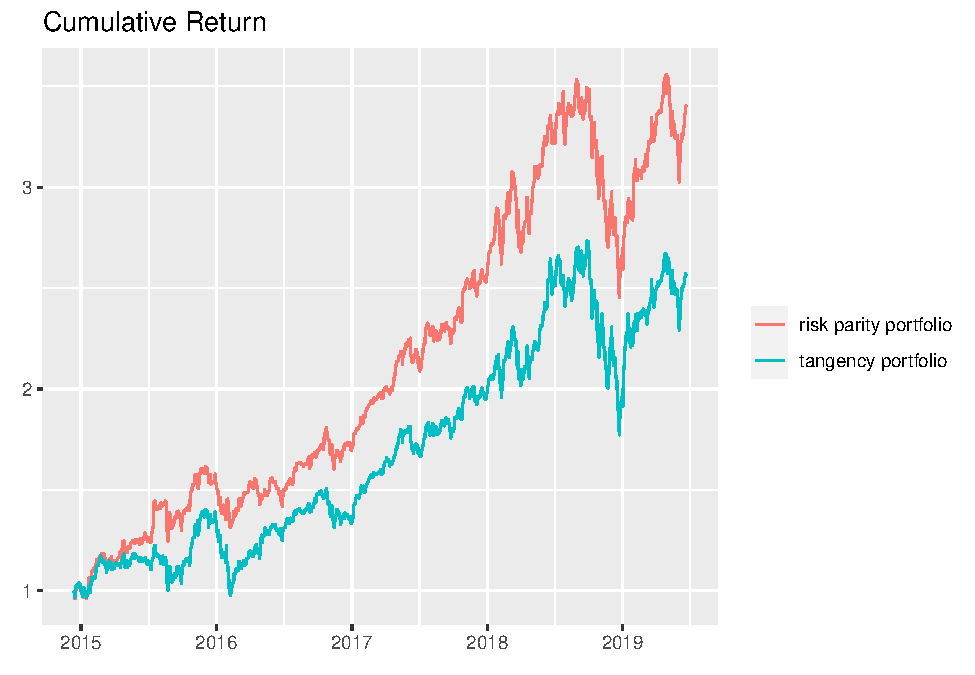
\includegraphics{TP-4_files/figure-latex/unnamed-chunk-7-1.pdf}
\caption{Rendement cumulé}
\end{figure}

\begin{figure}
\centering
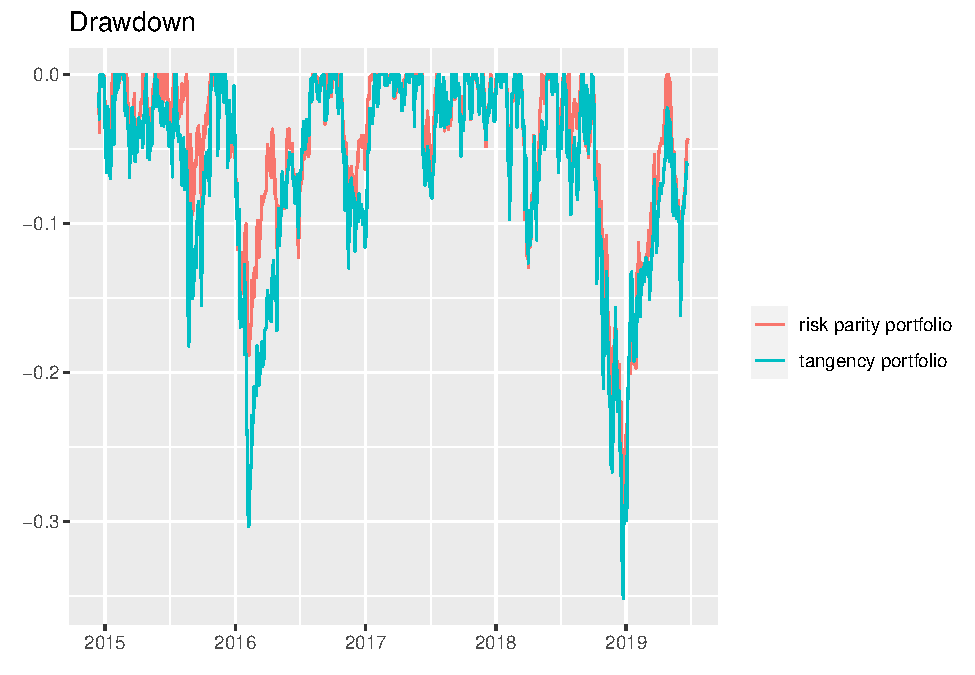
\includegraphics{TP-4_files/figure-latex/unnamed-chunk-8-1.pdf}
\caption{Perte maximale cumulée}
\end{figure}

\begin{figure}
\centering
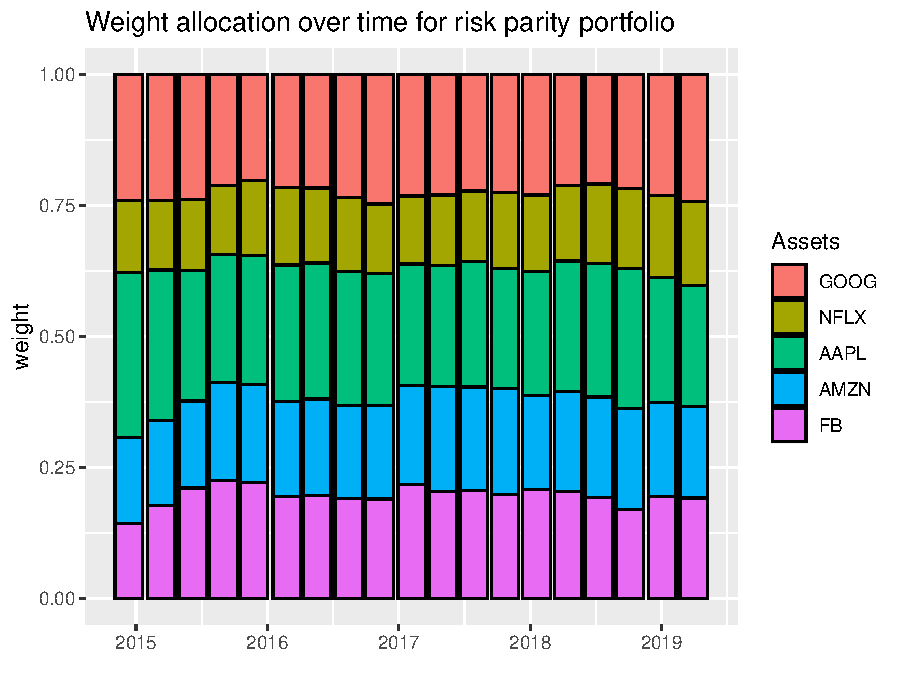
\includegraphics{TP-4_files/figure-latex/unnamed-chunk-9-1.pdf}
\caption{Composition du portefeuille Risk Parity}
\end{figure}

\begin{figure}
\centering
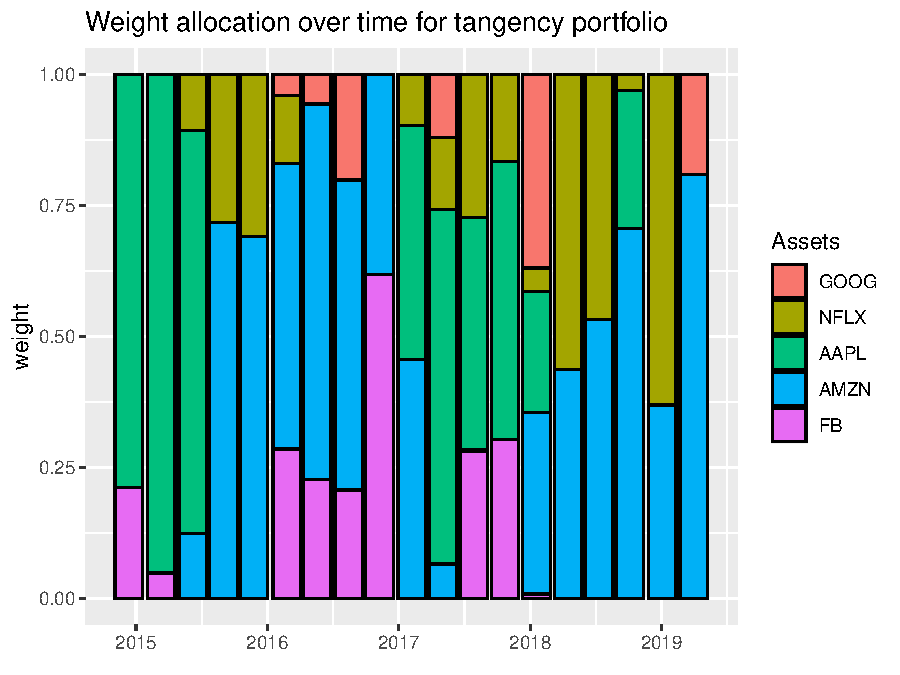
\includegraphics{TP-4_files/figure-latex/unnamed-chunk-10-1.pdf}
\caption{Composition du portefeuille tangent}
\end{figure}

\hypertarget{question-1}{%
\subsection{Question 1}\label{question-1}}

Que penser de l'algorithme ``Portefeuille Tangent,'' tel qu'il est
présenté?

La frontière efficiente en présence d'un taux sans risque est la
solution du problème:

\[
\begin{aligned}
    & \mbox{min}_w \ \   w^T \Sigma w \\
    \mbox{s.t.} & \\
    & \left(1- w^T \mathbf{1} \right) r_f + w^T \mu = \mu^* \\
\end{aligned}
\]

ou bien,

\[
\begin{aligned}
    & \mbox{min}_w \ \   w^T \Sigma w \\
    \mbox{s.t.} & \\
    & w^T (\mu - r_f) = \mu^* -r_f\\
\end{aligned}
\]

L'algorithme proposé dans la vignette résoud par contre:

\[
\begin{aligned}
    & \mbox{min}_w \ \   w^T \Sigma w \\
    \mbox{s.t.} & \\
    & w^T \mu = 1 \\
\end{aligned}
\]

\begin{itemize}
\tightlist
\item
  Que penser de cette formulation de la contrainte?
\item
  A l'aide des données fournies, modifier l'algorithme de calcul du
  portefeuille tangent pour y incorporer le taux sans risque.
\end{itemize}

On utilisera les données quotidiennes ci-dessous:

\begin{Shaded}
\begin{Highlighting}[]
\NormalTok{daily.price.file }\OtherTok{\textless{}{-}} \FunctionTok{file.path}\NormalTok{(}\FunctionTok{get.data.folder}\NormalTok{(), }\StringTok{"daily.price.rda"}\NormalTok{)}
\NormalTok{tickers }\OtherTok{\textless{}{-}} \FunctionTok{c}\NormalTok{(}\StringTok{"AAPL"}\NormalTok{, }\StringTok{"AMZN"}\NormalTok{, }\StringTok{"MSFT"}\NormalTok{, }\StringTok{"F"}\NormalTok{, }\StringTok{"SPY"}\NormalTok{, }\StringTok{"QQQ"}\NormalTok{, }\StringTok{"XOM"}\NormalTok{, }\StringTok{"MMM"}\NormalTok{, }\StringTok{"HD"}\NormalTok{, }\StringTok{"PG"}\NormalTok{, }\StringTok{"KO"}\NormalTok{)}
\FunctionTok{load}\NormalTok{(daily.price.file)}
\end{Highlighting}
\end{Shaded}

\begin{Shaded}
\begin{Highlighting}[]
\FunctionTok{kable}\NormalTok{(}\FunctionTok{table.Stats}\NormalTok{(daily.price), }\StringTok{"latex"}\NormalTok{, }\AttributeTok{booktabs=}\NormalTok{T) }\SpecialCharTok{\%\textgreater{}\%} \FunctionTok{kable\_styling}\NormalTok{(}\AttributeTok{latex\_options=}\StringTok{"scale\_down"}\NormalTok{)}
\end{Highlighting}
\end{Shaded}

\begin{table}[H]
\centering
\resizebox{\linewidth}{!}{
\begin{tabular}{lrrrrrrrrrrr}
\toprule
  & AAPL & AMZN & MSFT & F & SPY & QQQ & XOM & MMM & HD & PG & KO\\
\midrule
Observations & 3321.0000 & 3321.0000 & 3321.0000 & 3321.0000 & 3321.0000 & 3321.0000 & 3321.0000 & 3321.0000 & 3321.0000 & 3321.0000 & 3321.0000\\
NAs & 0.0000 & 0.0000 & 0.0000 & 0.0000 & 0.0000 & 0.0000 & 0.0000 & 0.0000 & 0.0000 & 0.0000 & 0.0000\\
Minimum & 9.6973 & 35.0300 & 11.6992 & 0.8857 & 54.5030 & 22.8605 & 37.1800 & 31.2938 & 13.5836 & 31.2946 & 11.9506\\
Quartile 1 & 30.0627 & 128.7100 & 21.9155 & 7.0687 & 107.3243 & 44.1221 & 57.0398 & 63.2295 & 26.7335 & 46.6560 & 18.8612\\
Median & 70.6362 & 291.5300 & 29.1490 & 9.2326 & 147.3649 & 70.5771 & 67.4404 & 96.7806 & 65.7329 & 63.5887 & 31.8386\\
\addlinespace
Arithmetic Mean & 87.0904 & 558.1350 & 46.7603 & 8.6546 & 163.4799 & 88.7199 & 64.8287 & 111.2979 & 83.2501 & 64.2153 & 30.6515\\
Geometric Mean & 62.0823 & 313.3150 & 37.0544 & 8.1115 & 149.5086 & 75.2676 & 63.9943 & 98.5782 & 60.0251 & 61.2222 & 28.5166\\
Quartile 3 & 117.9156 & 785.4100 & 56.9411 & 10.6602 & 206.2243 & 115.2020 & 72.8530 & 158.7457 & 124.6016 & 76.0785 & 38.8152\\
Maximum & 327.2000 & 2170.2200 & 188.1860 & 13.3217 & 338.3400 & 236.9800 & 83.6346 & 241.5468 & 245.3783 & 127.1400 & 59.6072\\
SE Mean & 1.1695 & 10.2363 & 0.6353 & 0.0484 & 1.2033 & 0.8937 & 0.1760 & 0.9326 & 1.1112 & 0.3621 & 0.1957\\
\addlinespace
LCL Mean (0.95) & 84.7973 & 538.0649 & 45.5146 & 8.5598 & 161.1205 & 86.9677 & 64.4835 & 109.4695 & 81.0714 & 63.5054 & 30.2679\\
UCL Mean (0.95) & 89.3835 & 578.2052 & 48.0060 & 8.7495 & 165.8393 & 90.4722 & 65.1738 & 113.1263 & 85.4288 & 64.9252 & 31.0352\\
Variance & 4542.4779 & 347982.1789 & 1340.5529 & 7.7716 & 4808.9586 & 2652.5974 & 102.9258 & 2888.1092 & 4100.7558 & 435.3391 & 127.1347\\
Stdev & 67.3979 & 589.9001 & 36.6136 & 2.7878 & 69.3467 & 51.5034 & 10.1452 & 53.7411 & 64.0371 & 20.8648 & 11.2754\\
Skewness & 1.0491 & 1.2531 & 1.5910 & -0.7300 & 0.5815 & 0.8034 & -0.4358 & 0.4329 & 0.7527 & 0.9931 & 0.1635\\
\addlinespace
Kurtosis & 0.6977 & 0.1875 & 1.7261 & -0.0735 & -0.8040 & -0.4726 & -0.8648 & -1.1710 & -0.6785 & 0.6805 & -0.8499\\
\bottomrule
\end{tabular}}
\end{table}

Le taux sans risque est fourni à une périodicité mensuelle:

\begin{Shaded}
\begin{Highlighting}[]
\NormalTok{tmp }\OtherTok{\textless{}{-}} \FunctionTok{read.csv}\NormalTok{(}\StringTok{"DP\_LIVE\_01032020211755676.csv"}\NormalTok{, }\AttributeTok{header=}\ConstantTok{TRUE}\NormalTok{, }\AttributeTok{sep=}\StringTok{";"}\NormalTok{)[, }\FunctionTok{c}\NormalTok{(}\StringTok{"TIME"}\NormalTok{, }\StringTok{"Value"}\NormalTok{)]}
\NormalTok{dt }\OtherTok{\textless{}{-}} \FunctionTok{ymd}\NormalTok{(}\FunctionTok{paste}\NormalTok{(tmp}\SpecialCharTok{$}\NormalTok{TIME, }\StringTok{"{-}01"}\NormalTok{, }\AttributeTok{sep=}\StringTok{""}\NormalTok{))}\SpecialCharTok{{-}}\DecValTok{1}
\NormalTok{rf\_rate }\OtherTok{\textless{}{-}} \FunctionTok{xts}\NormalTok{(tmp}\SpecialCharTok{$}\NormalTok{Value}\SpecialCharTok{/}\FloatTok{100.0}\NormalTok{, dt)}
\FunctionTok{colnames}\NormalTok{(rf\_rate) }\OtherTok{\textless{}{-}} \StringTok{"Rf"}
\NormalTok{show\_index }\OtherTok{\textless{}{-}} \FunctionTok{c}\NormalTok{(}\FunctionTok{head}\NormalTok{(}\FunctionTok{index}\NormalTok{(rf\_rate)), }\FunctionTok{tail}\NormalTok{(}\FunctionTok{index}\NormalTok{(rf\_rate)))}
\NormalTok{rf\_rate[show\_index,]}
\end{Highlighting}
\end{Shaded}

\begin{verbatim}
##                Rf
## 1964-05-31 0.0386
## 1964-06-30 0.0387
## 1964-07-31 0.0385
## 1964-08-31 0.0387
## 1964-09-30 0.0394
## 1964-10-31 0.0399
## 2019-07-31 0.0206
## 2019-08-31 0.0203
## 2019-09-30 0.0188
## 2019-10-31 0.0177
## 2019-11-30 0.0176
## 2019-12-31 0.0165
\end{verbatim}

A l'intérieur de la fonction \texttt{max\_sharpe\_ratio}, il faut
interpoler le taux sans risque correspondant à la date de calcul
(dernière date du tableau \texttt{dataset\$adjusted}). Vous pouvez
utiliser la function \texttt{approx} pour cela.

\hypertarget{question-2}{%
\subsection{Question 2}\label{question-2}}

Comparez la solution au portefeuille ``1/N,'' ou la richesse est allouée
uniformement à tous les actifs.

\end{document}
